\chapter{Complex Analysis}

%%%%%%%%%%%%%%%%%%%%%%%%%%%%%%%%%%%%%%%%%%%%%%%%%%%%%%%
\section{Jordan's Lemma}
We will need Jordan's lemma to calcuate the inverse Laplace transform using
contour integration. First we prove an useful lemma

%%%%%%%%%%%%%%%%%%
\begin{lemma} \label{L:sine}
If $0\le \theta \le \pi/2$, then
\begin{equation}
  \frac{\sin{\theta}}{\theta} \ge \frac{2}{\pi}.
\end{equation}
\end{lemma}
\begin{proof}
We only need to verify that function $\sin{x}/x$ is a decreading function, 
i.e. to verify the first derivate
\[
  \frac{d}{dx} \frac{\sin{x}}{x} = \frac{x\cos{x}-\sin{x}}{x^2}
\]
is non-positive. This can be proved by investgating the derivative of the
numerator
\[
  \frac{d}{dx} (x\cos{x}-\sin{x}) = -x\sin{x} \le 0.
\]
\end{proof}

Now the (generalized) Jordan's lemma,
%%%%%%%%%%%%%%%%%%
\begin{lemma}[Generalized Jordan's Lemma] \label{L:jordan}
\footnote{Adapted from Hayek, Advanced Mathematical Methods in Science and
    Engineering, 5.16.1, and F. Boesch's slide No. 10.}
Let $\alpha$, $b$, and $c$ be real numbers, and $b>0$, also let $C_R$ be a 
contour with radius $R$ and 
$\frac{\pi}{2}-c-\beta\le\theta\le\frac{3\pi}{2}-c+\beta$, where 
$\beta$ is determined by equation $\alpha=R\sin{\beta}$, and 

%%%%%%%%%%%%%%%%%%%%%%%%%%%%%%%%%%%%
\begin{figure} \label{F:cont1}
  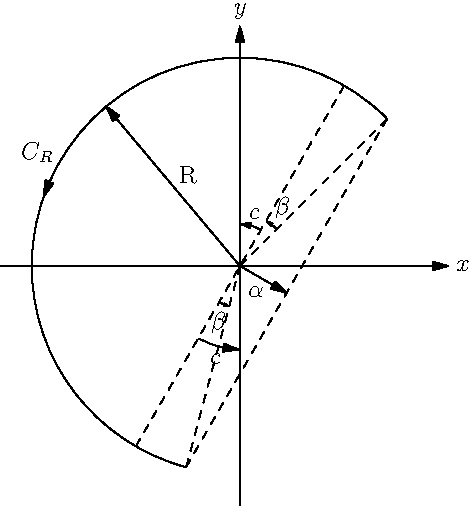
\includegraphics[width=3in]{graphics/contour_jordan.pdf}
\end{figure}
%%%%%%%%%%%%%%%%%%%%%%%%%%%%%%%%%%%%

\[
  I=\int_{C_R} e^{(be^{ic}) z} f(z) dz,
\]
then
\begin{equation} \label{E:jordan1}
  |I|\le \max_z |f(z)| \times \pi 
         \left[ \alpha e^{b\alpha}+\frac{1-e^{-bR}}{b} \right]
         \qquad \alpha\ge 0,
\end{equation}
and 
\begin{equation} \label{E:jordan2}
  |I|\le \max_z |f(z)| \times \frac{\pi}{b}
         \left[ e^{\frac{2b\alpha}{\pi}} - e^{-bR} \right]
         \qquad \alpha<0.
\end{equation}
Specifically, if $\max_z |f(z)|\to 0$ as $R\to \infty$, then
\[
  \lim_{R\to \infty} I = 0.
\]
\end{lemma}
%%%%%%%%%%%%%%%%%%%%%%%%%%%%%%%%%%
\begin{proof}
From definition we have
\[
  I=\int_{\frac{\pi}{2}-c-\beta}^{\frac{3\pi}{2}-c+\beta}
    e^{bRe^{i(\theta+c)}} f(Re^{i\theta}) iRe^{i\theta} d\theta,
\]
hence
\[
  |I| \le \max_{\theta}|f(Re^{i\theta})| \times R
          \int_{\frac{\pi}{2}-\beta}^{\frac{3\pi}{2}+\beta}
            e^{bR\cos{\theta}} d\theta
      = \max_{\theta}|f(Re^{i\theta})| \times R \times J
\]
where 
\[
  J= \int_{\frac{\pi}{2}-\beta}^{\frac{3\pi}{2}+\beta}
       e^{bR\cos{\theta}} d\theta.
\]

We first investigate the case with $\beta\ge0$ (or equivalently
$\alpha\ge 0$), note that in this case
\[
  J=\left( 
      \int_{\frac{\pi}{2}-\beta}^{\frac{\pi}{2}}
      + \int_{\frac{\pi}{2}}^{\frac{3\pi}{2}}
      + \int_{\frac{3\pi}{2}}^{\frac{3\pi}{2}+\beta}
    \right)
    e^{bR\cos{\theta}} d\theta,
\]
it is easy to see that (using variable transformation)
\[
  J= 2\int_0^{\beta} e^{bR\sin{\theta}} d\theta
      + \int_0^{\pi} e^{-bR\sin{\theta}} d\theta.
\]
Now using the fact that $\alpha=R\sin{\beta}$ and lemma \ref{L:sine} we get
\[
  \int_0^{\beta} e^{bR\sin{\theta}} d\theta
  \le \int_0^{\beta} e^{bR\sin{\beta}} d\theta
  = \beta e^{bR\sin{\beta}} \le \frac{\pi\alpha}{2R} e^{b\alpha}.
\]
And again using lemma \ref{L:sine} we get
\[
  \int_0^{\pi} e^{-bR\sin{\theta}} d\theta
  = 2\int_0^{\frac{\pi}{2}} e^{-bR\sin{\theta}} d\theta
  \le 2\int_0^{\frac{\pi}{2}} e^{-bR\frac{2\theta}{\pi}} d\theta
  = \frac{\pi}{bR} (1-e^{-bR}).
\]
Substitue these back, we get inequality \ref{E:jordan1}.

Next we look at the case with $\beta<0$ (or equivalently $\alpha<0$). We have
\[
  J= \int_{\frac{\pi}{2}-\beta}^{\frac{3\pi}{2}+\beta}
       e^{bR\cos{\theta}} d\theta
   = \int_{-\beta}^{\pi+\beta} e^{-bR\sin{\theta}} d\theta
   = 2 \int_{-\beta}^{\frac{\pi}{2}} e^{-bR\sin{\theta}} d\theta,
\]
Using Lemma \ref{L:sine}, we have
\[
  J \le 2 \int_{-\beta}^{\frac{\pi}{2}} e^{-bR\frac{2\theta}{\pi}} d\theta
    = \frac{\pi}{bR}\left( e^{\frac{2b}{\pi} R\beta} - e^{-bR} \right).
\]
Using the fact that $R|\beta|\ge R\sin{|\beta|}$ hence 
$R\beta\le R\sin{\beta}=\alpha$, we get
\[
  J \le \frac{\pi}{bR}\left( e^{\frac{2b\alpha}{\pi}} - e^{-bR} \right),
\]
and thus inequality \ref{E:jordan2}.
\end{proof}

A useful corollary for doing inverse Laplace transform is the following:
%%%%%%%%%%%%%%%%%%%%%%%%%%%
\begin{corollary} \label{C:jordan}
Let $b>0$ and let $C_R$ be a contour with radius $R$ and 
$\frac{\pi}{2}-\beta \le \theta \le \frac{3\pi}{2}+\beta$, 
if 
\[
	\lim_{R\to\infty} \max_z |f(z)| = 0,
\]
then

%%%%%%%%%%%%%%%%%%%%%%%%%%%%%%%%%%%%%%%%%
\begin{marginfigure} \label{F:cont_jordan2}
  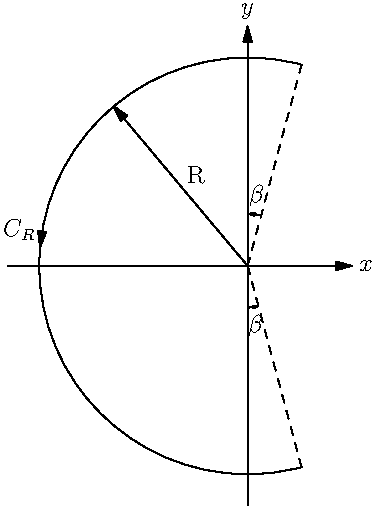
\includegraphics{graphics/contour_jordan2.pdf}
%	\caption{Contour.}
\end{marginfigure}
%%%%%%%%%%%%%%%%%%%%%%%%%%%%%%%%%%%%%%%%%

\[
  \lim_{R\to \infty} \int_{C_R} e^{b z} f(z) dz = 0.
\]
\end{corollary}
\begin{proof}
	Directly from the generalized Jordan's lemma \ref{L:jordan} with $c=0$.
\end{proof}



%%%%%%%%%%%%%%%%%%%%%%%%%%%
\begin{remark}
Here we give several special cases of the Jordan's Lemma above. Here we assume
$\max_z |f(z)|\to 0$ as $R\to \infty$, and $\beta=0$.
\begin{enumerate}
\item If $c=\pi/2$, we have
      \[
        \lim_{R\to \infty} \int_{C_R} e^{ibz} f(z) dz = 0,
      \]
      where $C_R$ is an arc in the first and/or the second quadrants.
\item If $c=-\pi/2$, we have
      \[
        \lim_{R\to \infty} \int_{C_R} e^{-ibz} f(z) dz = 0,
      \]
      where $C_R$ is an arc in the third and/or the fourth quadrants.
\item If $c=0$, we have
      \[
        \lim_{R\to \infty} \int_{C_R} e^{bz} f(z) dz = 0,
      \]
      where $C_R$ is an arc in the second and/or the third quadrants.
\item If $c=\pi$, we have
      \[
        \lim_{R\to \infty} \int_{C_R} e^{-bz} f(z) dz = 0,
      \]
      where $C_R$ is an arc in the fourth and/or the first quadrants.
\end{enumerate}
\end{remark}
